\begin{frame}{Real Camera Noise Is Not Gaussian}
  \begin{center}
    \resizebox{\textwidth}{!}{%
    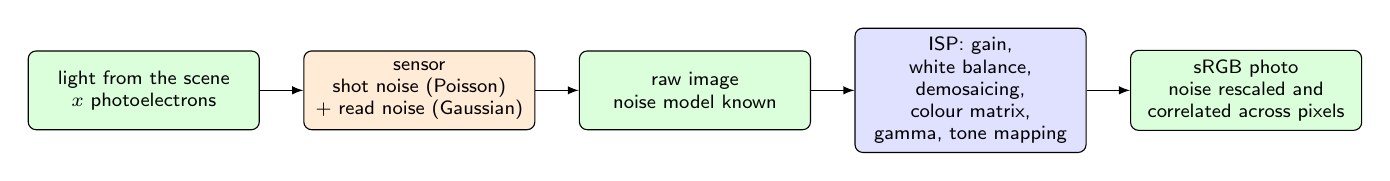
\begin{tikzpicture}[font=\sffamily\scriptsize, >=latex,
        stage/.style={draw, rounded corners=0.1cm, align=center, minimum height=1.0cm, text width=2.7cm},
        lightbox/.style={stage, fill=green!14}, sensbox/.style={stage, fill=orange!16}, ispbox/.style={stage, fill=blue!12}]
      \node[lightbox] (scene)  at (0,0)    {light from the scene\\$x$ photoelectrons};
      \node[sensbox]  (sensor) at (3.5,0)  {sensor\\shot noise (Poisson)\\+ read noise (Gaussian)};
      \node[lightbox] (raw)    at (7.0,0)  {raw image\\noise model known};
      \node[ispbox]   (isp)    at (10.5,0) {ISP: gain, white balance,\\demosaicing, colour matrix,\\gamma, tone mapping};
      \node[lightbox] (srgb)   at (14.0,0) {sRGB photo\\noise rescaled and\\correlated across pixels};
      \draw[->] (scene) -- (sensor);
      \draw[->] (sensor) -- (raw);
      \draw[->] (raw) -- (isp);
      \draw[->] (isp) -- (srgb);
    \end{tikzpicture}}
  \end{center}
  \vspace{-0.6em}
  \begin{itemize}\footnotesize\itemsep0.3em
    \item \textbf{Raw sensor noise is well understood.} Shot noise is Poisson with mean equal to the true light $x$; read noise is zero-mean Gaussian with fixed variance. Together they act as one heteroscedastic Gaussian, $y \sim \mathcal{N}(x,\ \lambda_{\text{read}} + \lambda_{\text{shot}}\,x)$, where $y$ is the observed raw value and the two $\lambda$ are set by the camera's analog and digital gains.
    \item \textbf{The image signal processor (ISP) reshapes it.} Gain, white balance, colour correction and gamma rescale the noise and pass it through nonlinearities, and demosaicing correlates it across neighbouring pixels.
    \item \textbf{Synthetic Gaussian training does not transfer.} Denoising autoencoders trained on added white Gaussian noise (covered earlier) assume the model a phone camera violates; on real-noise benchmarks, learned methods trained on synthetic noise lost to the classical BM3D filter.
    \item \textbf{SIDD} (Smartphone Image Denoising Dataset) is a standard real-noise benchmark: about 30{,}000 noisy images of 10 scenes from five phones, with estimated ground truth.
  \end{itemize}
  {\scriptsize Brooks et al., CVPR 2019, \href{https://arxiv.org/abs/1811.11127v1}{arXiv:1811.11127v1}, Sec.~2 and 3.1, Eq.~(1); Abdelhamed et al., CVPR 2018, \href{https://openaccess.thecvf.com/content_cvpr_2018/html/Abdelhamed_A_High-Quality_Denoising_CVPR_2018_paper.html}{CVF Open Access}.\par}
\end{frame}

\begin{frame}{Restormer and NAFNet: Standard Backbones}
  \begin{columns}[T,onlytextwidth]
    \column{0.55\textwidth}
      \begin{itemize}\footnotesize\itemsep0.3em
        \item \textbf{Restormer} (CVPR 2022) computes self-attention across channels: queries, keys and values come from $1{\times}1$ and depth-wise $3{\times}3$ convolutions, the attention map is $C \times C$ for $C$ channels, and cost grows linearly with image size. 40.02\,dB PSNR on SIDD, the only one above 40\,dB in its comparison.
        \item \textbf{NAFNet} (ECCV 2022): a plain U-Net (covered earlier) without nonlinear activation functions. Its SimpleGate splits the channels into halves $X$ and $Y$ and outputs $X \odot Y$, itself a nonlinearity. 40.30\,dB on SIDD and 33.69\,dB on the GoPro deblurring benchmark (below), at 8.4\% of the compute of the previous best GoPro model.
        \item \textbf{What still wins on PSNR in 2026.} NTIRE 2026 denoising (Gaussian noise, standard deviation $\sigma = 50$; 20 finalists of 116 registrants): the top four finished within 0.03\,dB. Leaders kept Restormer and MambaIR backbones (the winners fused them with HAT) and gained from more data, patches grown from 128 to 768 pixels, and test-time flip and rotation averaging; diffusion models still trail on PSNR.
      \end{itemize}
    \column{0.43\textwidth}
      \centering
      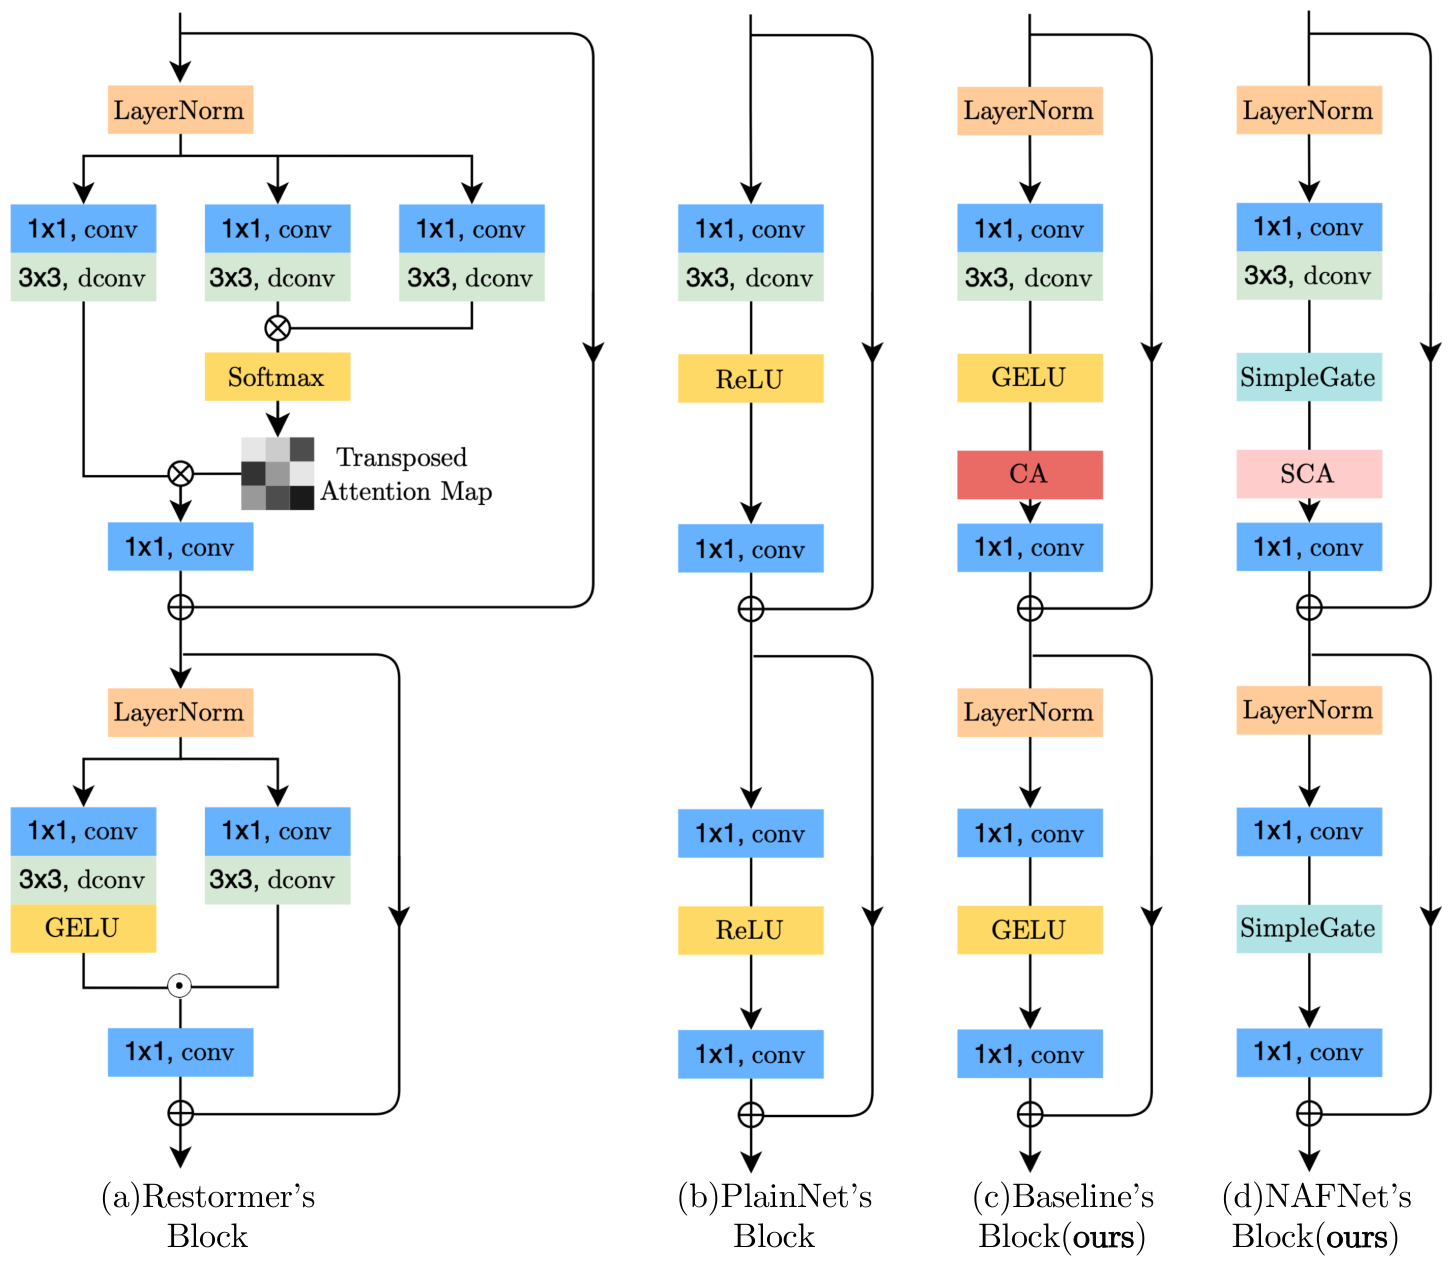
\includegraphics[width=\linewidth,height=0.52\textheight,keepaspectratio]{images/image-restoration-applications/nafnet_fig3_block_comparison.png}\\[0.2em]
      {\scriptsize (a) Restormer block, (d) NAFNet block. Chen et al., ``Simple Baselines for Image Restoration,'' ECCV 2022, \href{https://arxiv.org/abs/2204.04676v4}{arXiv:2204.04676v4}, Figure~3.\par}
  \end{columns}
  \vspace{-0.3em}
  {\scriptsize Restormer: \href{https://arxiv.org/abs/2111.09881v2}{arXiv:2111.09881v2}, Table~6; NTIRE 2026: \href{https://arxiv.org/abs/2606.16031v1}{arXiv:2606.16031v1}, Secs.~4, 5.3.\par}
\end{frame}

\begin{frame}{Training a Denoiser Without Clean Images}
  \begin{columns}[T,onlytextwidth]
    \column{0.55\textwidth}
      \begin{itemize}\footnotesize\itemsep0.3em
        \item \textbf{Clean targets are often unavailable.} A noise-free photo needs a long exposure, fully sampled magnetic resonance imaging (MRI) rules out moving subjects, and in biomedical microscopy even a second noisy capture of the same sample is often impossible.
        \item \textbf{Noise2Noise} trains on two independent noisy copies $y_1 = x + n_1$ and $y_2 = x + n_2$ of the same clean image $x$. If $n_2$ has zero mean and is independent of $x$ and $n_1$,
        \[ \mathbb{E}\,\|f_\theta(y_1) - y_2\|^2 = \mathbb{E}\,\|f_\theta(y_1) - x\|^2 + \mathbb{E}\,\|n_2\|^2 , \]
        so the denoiser $f_\theta$ has the same optimum as with clean targets. On Kodak with Gaussian noise ($\sigma = 25$): 32.50\,dB with clean targets, 32.48\,dB with noisy ones.
        \item \textbf{Noise2Void} needs only single noisy images. A blind-spot network (right, b) predicts each pixel from its neighbours without seeing the pixel itself, so it cannot copy the noise. This works when the noise is independent across pixels given the signal, while the signal is not.
      \end{itemize}
      {\scriptsize Lehtinen et al., ICML 2018, \href{https://arxiv.org/abs/1803.04189v3}{arXiv:1803.04189v3}, Sec.~1--2, Table~1; Krull et al., Sec.~1.\par}
    \column{0.43\textwidth}
      \centering
      \vspace{0.8em}
      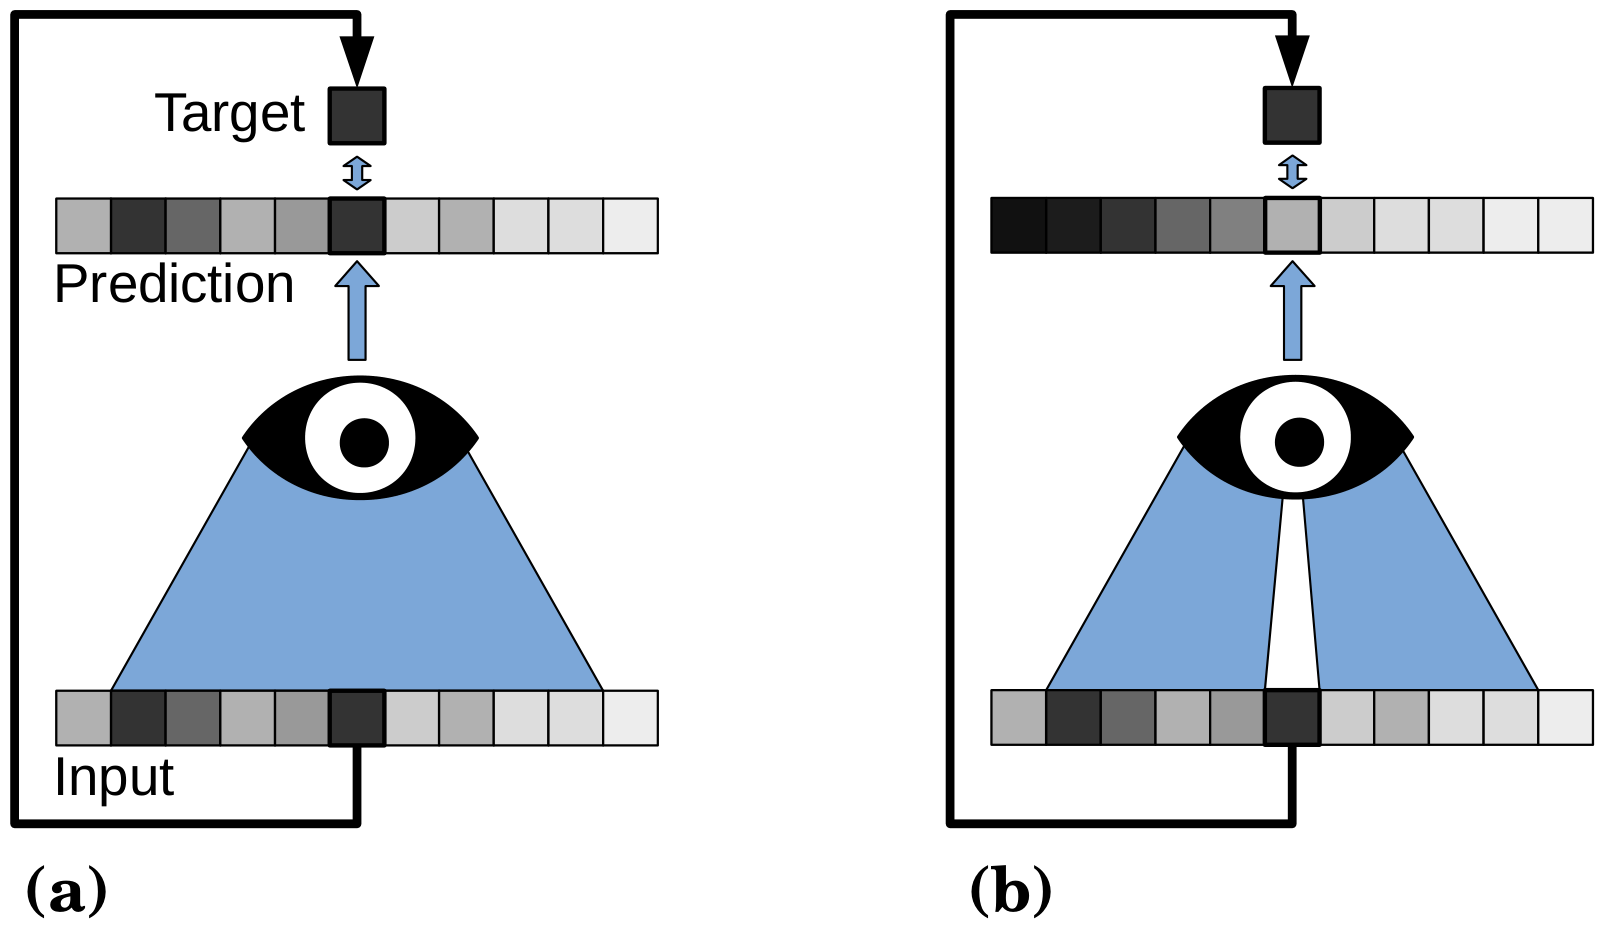
\includegraphics[width=\linewidth,height=0.46\textheight,keepaspectratio]{images/image-restoration-applications/noise2void_fig2_blind_spot.png}\\[0.2em]
      {\scriptsize (a) Ordinary network, (b) blind-spot network. Krull et al., ``Noise2Void - Learning Denoising from Single Noisy Images,'' CVPR 2019, \href{https://arxiv.org/abs/1811.10980v2}{arXiv:1811.10980v2}, Figure~2.\par}
  \end{columns}
\end{frame}

\begin{frame}{Deblurring: From Blur Kernels to State Spaces}
  \begin{columns}[T,onlytextwidth]
    \column{0.52\textwidth}
      \begin{itemize}\footnotesize\itemsep0.3em
        \item \textbf{Blur model} $y = k * x + n$: the kernel $k$ traces camera shake, object motion or a defocus disk, and $*$ is convolution. Non-blind deblurring knows $k$; blind deblurring infers it, and in dynamic scenes $k$ varies across the image.
        \item \textbf{Data.} GoPro averages 7--13 consecutive frames of 240\,fps video into one blurred frame (2,103 training, 1,111 test images); RealBlur tests real camera blur in raw-processed (R) and JPEG (J) sets.
        \item \textbf{Frequency domain.} After a fast Fourier transform (FFT), convolution becomes an element-wise product; FFTformer (CVPR 2023) computes attention that way: 34.21\,dB on GoPro.
        \item \textbf{State spaces.} Selective state-space layers (defined with MambaIR above) scan the flattened feature map in linear time. EVSSM (CVPR 2025) scans in one direction but flips or transposes the features before each scan: 34.51\,dB on GoPro, 34.34\,dB on RealBlur-J.
      \end{itemize}
    \column{0.46\textwidth}
      \centering
      \vspace{0.4em}
      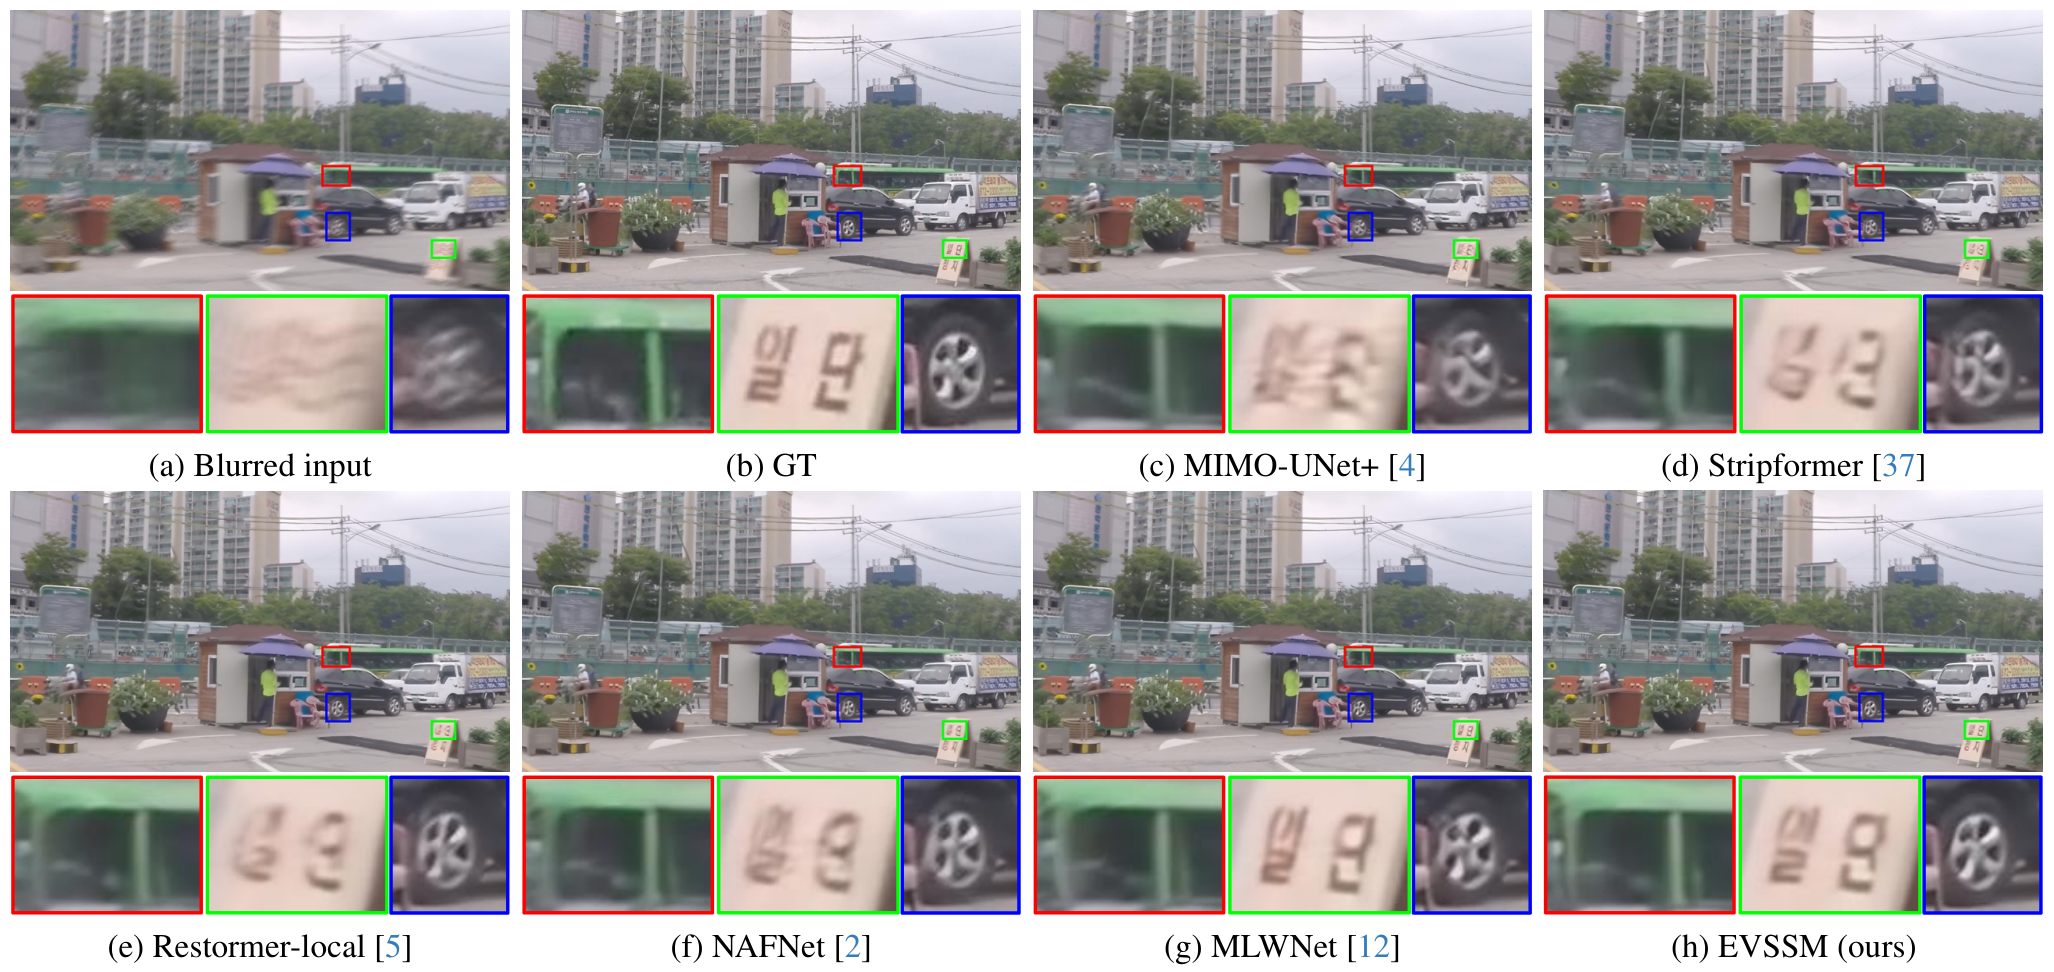
\includegraphics[width=\linewidth,height=0.5\textheight,keepaspectratio]{images/image-restoration-applications/evssm_fig2_gopro_deblurring.png}\\[0.2em]
      {\scriptsize GoPro test image: (a) blurred input, (b) ground truth, (h) EVSSM. Kong et al., ``Efficient Visual State Space Model for Image Deblurring,'' CVPR 2025, \href{https://arxiv.org/abs/2405.14343v2}{arXiv:2405.14343v2}, Figure~2, Tables~1--2.\par}
  \end{columns}
  {\scriptsize Nah et al., CVPR 2017, \href{https://openaccess.thecvf.com/content_cvpr_2017/html/Nah_Deep_Multi-Scale_Convolutional_CVPR_2017_paper.html}{CVF Open Access}, Secs.~2, 3.2, 4.1; Rim et al., ECCV 2020, \href{https://doi.org/10.1007/978-3-030-58595-2_12}{doi:10.1007/978-3-030-58595-2\_12}; Kong et al., CVPR 2023, \href{https://arxiv.org/abs/2211.12250v1}{arXiv:2211.12250v1}, Table~1.\par}
\end{frame}

\begin{frame}{All-in-One Restoration: Prompts and Instructions}
  \centering
  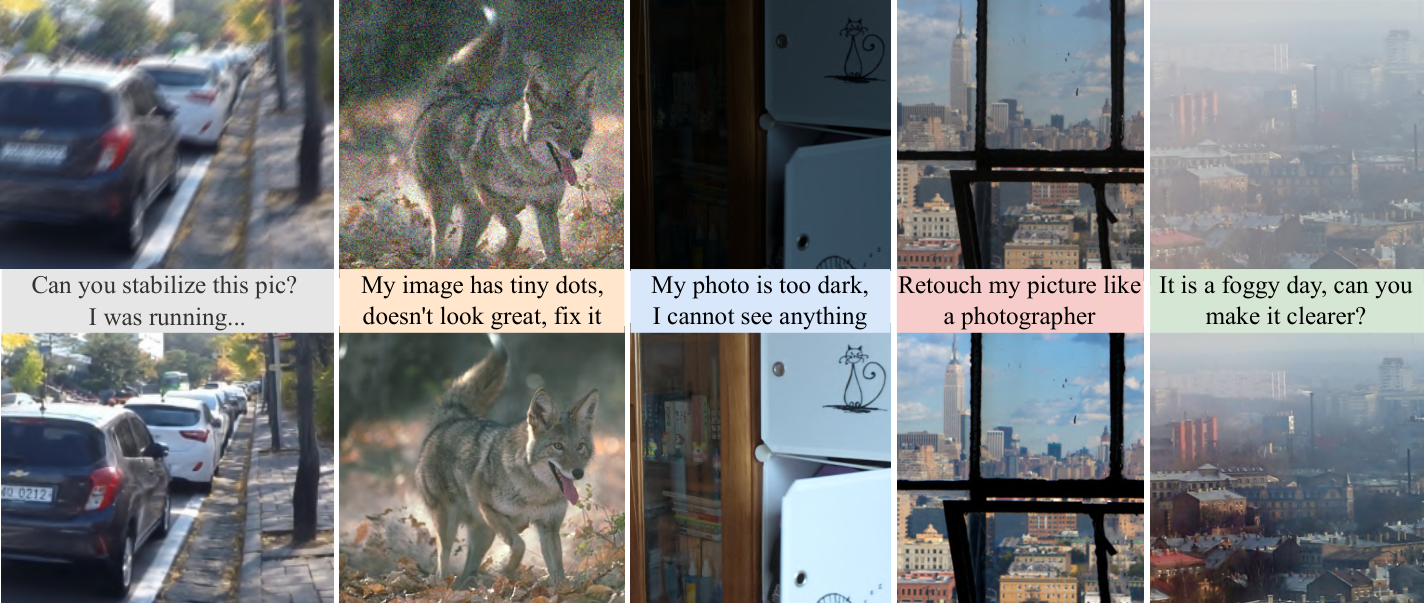
\includegraphics[width=\textwidth,height=0.25\textheight,keepaspectratio]{images/image-restoration-applications/instructir_fig1_instructions.png}\\[0.1em]
  {\scriptsize Typed instructions (middle row) steer one model. Conde et al., ``InstructIR: High-Quality Image Restoration Following Human Instructions,'' ECCV 2024, \href{https://arxiv.org/abs/2401.16468v5}{arXiv:2401.16468v5}, Figure~1.\par}
  \begin{columns}[T,onlytextwidth]
    \column{0.49\textwidth}
      \begin{itemize}\footnotesize\itemsep0.3em
        \item \textbf{PromptIR} (NeurIPS 2023): one network for several degradations. Learned prompt components, weighted by attention from the input's own features, are injected at several decoder stages.
        \item \textbf{DA-CLIP} (ICLR 2024): a trainable copy of CLIP's image encoder, attached through ControlNet-style zero-initialised connections (covered earlier), predicts which of 10 degradations is present and steers the frozen CLIP encoder to a clean-content embedding that guides a diffusion restorer.
      \end{itemize}
    \column{0.49\textwidth}
      \begin{itemize}\footnotesize\itemsep0.3em
        \item \textbf{InstructIR} (ECCV 2024): the user states the problem in words. A frozen sentence encoder (BGE-micro) and a learned projection embed it as $e$; each NAFNet block multiplies its channels by $m = \mathrm{sigmoid}(W e)$, so the text selects features.
        \item Trained on over 10{,}000 GPT-4-written prompts, one 16M-parameter model covers five to seven tasks, about 1\,dB above earlier all-in-one models.
      \end{itemize}
  \end{columns}
  {\scriptsize PromptIR: \href{https://arxiv.org/abs/2306.13090v1}{arXiv:2306.13090v1}; DA-CLIP: \href{https://arxiv.org/abs/2310.01018v2}{arXiv:2310.01018v2}.\par}
\end{frame}

\begin{frame}{Agentic Restoration: A VLM Plans the Toolchain}
  \begin{columns}[T,onlytextwidth]
    \column{0.55\textwidth}
      \begin{itemize}\footnotesize\itemsep0.3em
        \item \textbf{Order matters.} Denoising then dehazing works, dehazing first fails; deraining before super-resolution works, after it fails.
        \item \textbf{AgenticIR} (ICLR 2025): a fine-tuned VLM (DepictQA; VLMs covered earlier) names the degradations, GPT-4 orders the tools, a failed step is rolled back and re-planned, and past outcomes are kept as notes for the planner. The toolbox holds 3--6 specialist models for each of eight degradations.
        \item \textbf{4KAgent} (NeurIPS 2025): a VLM with image-quality experts plans; several expert models run per step and the best-scoring output is kept. Tested on 26 benchmarks in 11 task categories, including satellite, microscopy and X-ray images.
        \item \textbf{General image editors are no substitute.} GPT-Image restorations are ``often perceptually pleasant'' but change geometry, object positions or counts, and even perspective.
      \end{itemize}
    \column{0.43\textwidth}
      \centering
      \vspace{0.3em}
      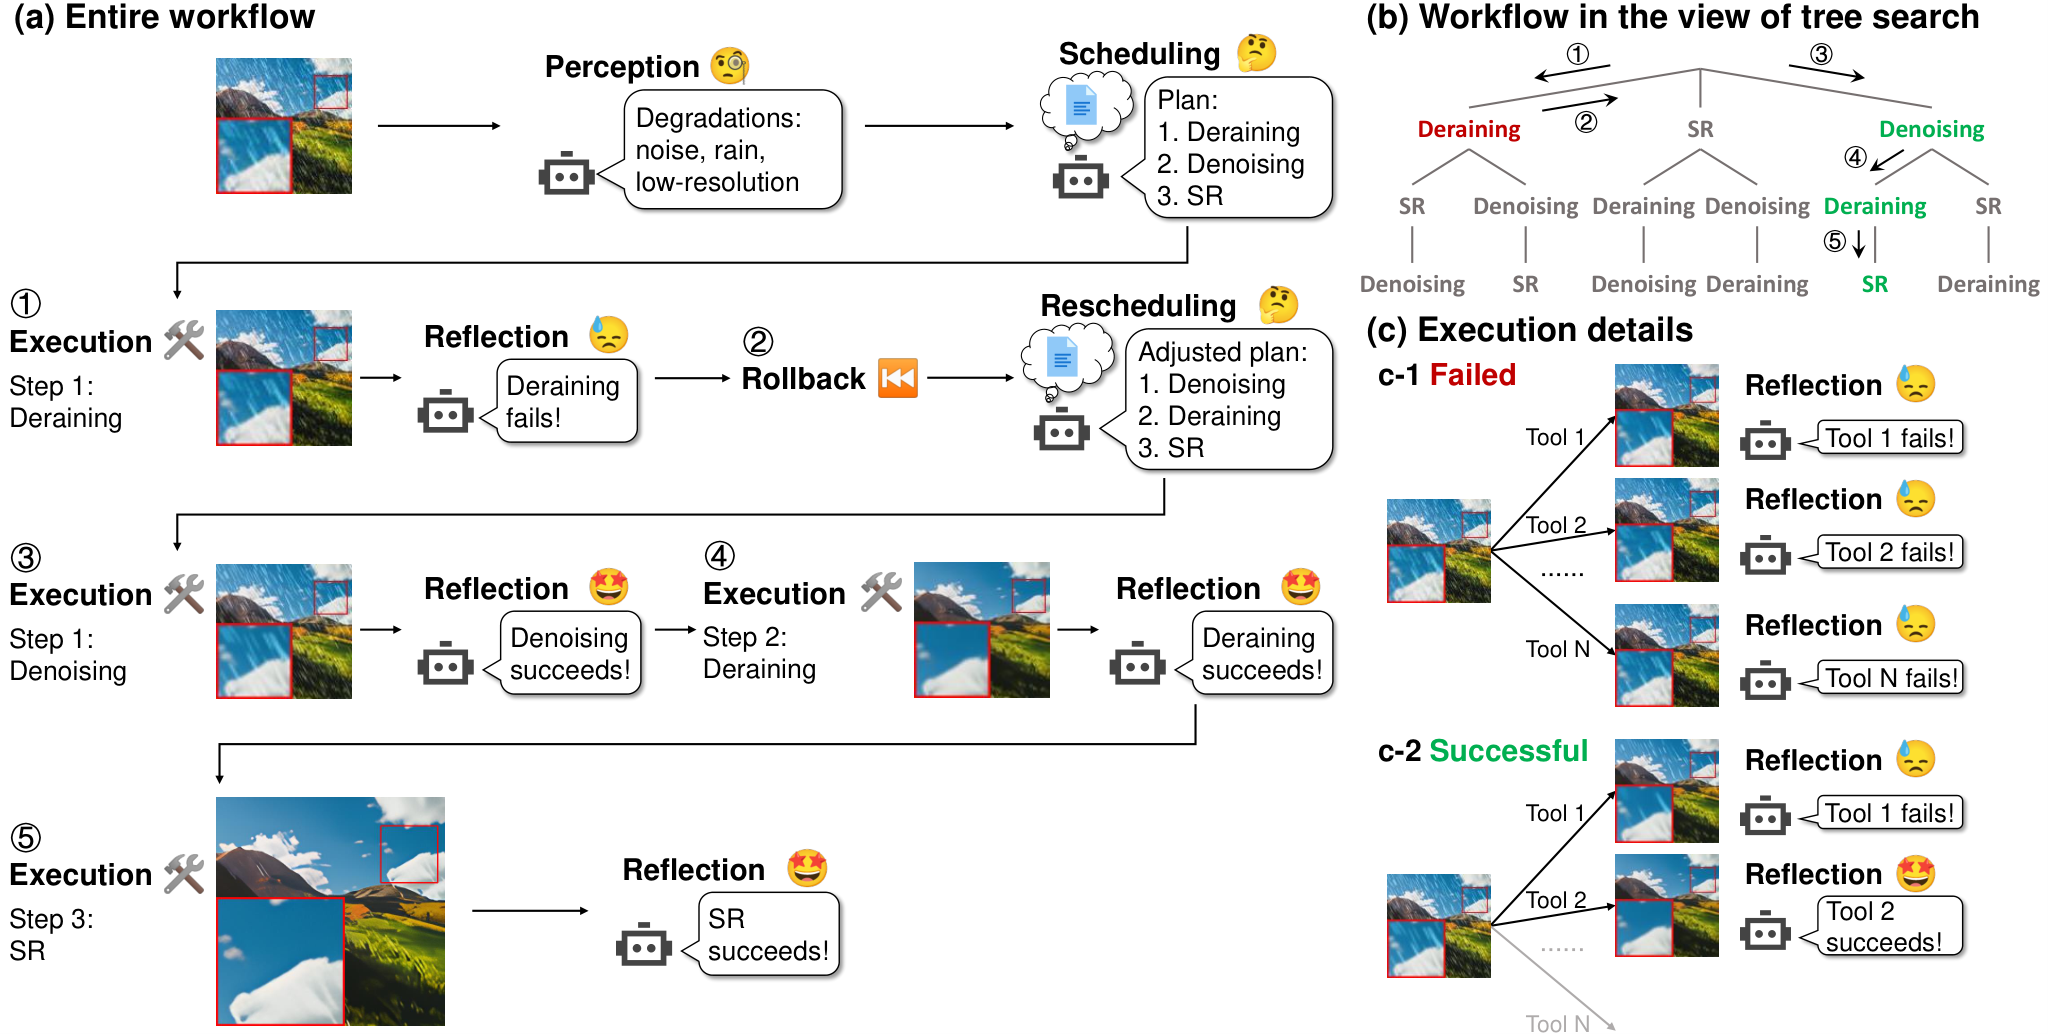
\includegraphics[width=\linewidth,height=0.5\textheight,keepaspectratio]{images/image-restoration-applications/agenticir_fig2_workflow.png}\\[0.2em]
      {\scriptsize Zhu et al., ``An Intelligent Agentic System for Complex Image Restoration Problems,'' ICLR 2025, \href{https://arxiv.org/abs/2410.17809v2}{arXiv:2410.17809v2}, Figure~2 (operation order: Figure~3).\par}
  \end{columns}
  {\scriptsize Zuo et al., NeurIPS 2025, \href{https://arxiv.org/abs/2507.07105v1}{arXiv:2507.07105v1}; Yang et al., ICME 2026, \href{https://arxiv.org/abs/2505.05621v3}{arXiv:2505.05621v3}.\par}
\end{frame}

\begin{frame}{Zero-Shot Restoration with a Generative Prior}
  \begin{itemize}\footnotesize\itemsep0.35em
    \item \textbf{Setup.} A measurement $y = \mathcal{A}(x) + n$ with a known operator $\mathcal{A}$ (blur, downsampling, a mask) and noise $n$. A diffusion model trained only on clean images supplies the prior $p(x)$; nothing is retrained per task.
    \item \textbf{Bayes in score form.} Sampling the posterior $p(x \mid y)$ needs
    \[ \nabla_{x_t} \log p_t(x_t \mid y) = \nabla_{x_t} \log p_t(x_t) + \nabla_{x_t} \log p_t(y \mid x_t), \]
    the score of the prior (covered earlier) plus a likelihood term that is intractable at intermediate noise levels $t$.
    \item \textbf{Diffusion posterior sampling (DPS)}, ICLR 2023, approximates $p(y \mid x_t) \approx p(y \mid \hat{x}_0)$, where $\hat{x}_0 = \mathbb{E}[x_0 \mid x_t]$ is the denoiser's clean estimate, and adds a gradient step after every reverse step:
    \[ x_{t-1} \leftarrow x'_{t-1} - \zeta_t \nabla_{x_t} \big\| y - \mathcal{A}(\hat{x}_0(x_t)) \big\|_2^2 , \]
    with $x'_{t-1}$ the ordinary reverse step and $\zeta_t$ a step size. One prior then serves super-resolution, deblurring and inpainting, and nonlinear operators such as non-uniform blur.
    \item \textbf{2025 refinements.} Decoupled annealing posterior sampling (DAPS, CVPR 2025) lets consecutive steps differ widely so later steps can undo early mistakes on hard nonlinear problems; PnP-Flow (ICLR 2025) uses a flow-matching model (covered earlier) as the denoiser in a plug-and-play loop of data-fidelity gradient steps, re-projection onto the flow path and denoising, without backpropagating through the ODE.
  \end{itemize}
  \vspace{0.1em}
  {\scriptsize Chung et al., ICLR 2023, \href{https://arxiv.org/abs/2209.14687v4}{arXiv:2209.14687v4}, Eqs.~(5), (11), (21), Algorithm~1; Zhang et al., CVPR 2025, \href{https://arxiv.org/abs/2407.01521v3}{arXiv:2407.01521v3}; Martin et al., ICLR 2025, \href{https://arxiv.org/abs/2410.02423v3}{arXiv:2410.02423v3}.\par}
\end{frame}
